\noindent
Graph algorithms are typically very memory-intensive while the memory access patterns are very random (i.e., poor sptial and temporal locality). 
These characteristics greatly reduce the efficiency of traditional memory systems that are typically optimized for serving sequential memory requests. 
For example, running BFS on a GPU, we observe that the memory system becomes the performance bottleneck even when HBM provides 512GB/s. 
In this project, we aim to implement a memory system that can support both random and sequential memory accesses for sparse and dense datasets.

\noindent
\textbf{On-chip Cache Architecture:} 
We propose \texttt{Elastic-Cache} to efficiently support both narrow- and wide-width data accesses from multiple non-contiguous memory locations to co-reside in a single cache line. 
We introduce a concept of chunk tags to store tags for narrow-width data blocks (e.g., 4-, 8-, or 16-byte byte blocks) along with a conventional tag (dubbed commong tag) for each cache line (Figure~\ref{fig:elastic-cache}). 
This adds only a small area overhead, but allow us to efficiently use 64-byte cache lines for storing narrow-width data blocks from non-contiguous addresses, as well as a 64-byte block whose bytes are from consecutive addresses.
Note that just adopting narrow cache lines is not efficient to handle sequential memory requests for dense datasets according to our experiments.
%Figure~\ref{fig:elastic-cache-flow} describes the access flow of the proposed \texttt{Elastic-Cache}. 
We will employ the proposed \texttt{Elastic-Cache} architecture for both private SRAM-based L1 and shared eDRAM-based L2 on-chip caches.

% shall I discuss a mechanism to minimize cache interference by irregular/random accesses?

\begin{wrapfigure}{r}[0pt]{0.4\textwidth}
\center
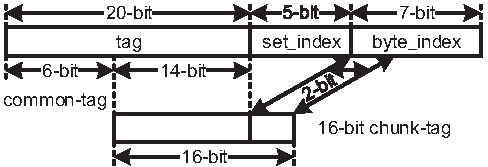
\includegraphics[width=1.0\linewidth]{./fig/chunk_tag_16bit-eps-converted-to.pdf}
\caption{The chunk and common tags to support both narrow- and wide-width on-chip cache accesses for a 4-way 16KB cache.}
\label{fig:elastic-cache}
\end{wrapfigure}

\begin{comment}
\begin{wrapfigure}{r}[0pt]{0.4\textwidth}
\center
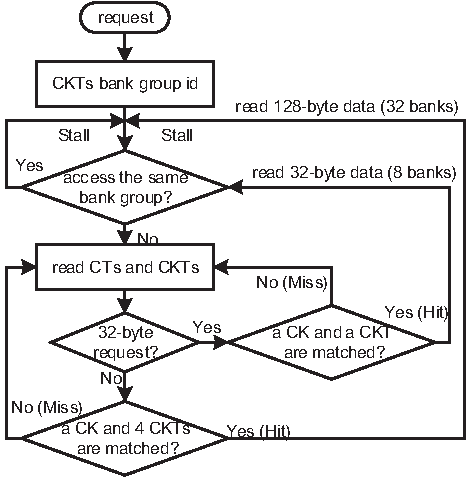
\includegraphics[width=1.0\linewidth]{./fig/flow_chart-eps-converted-to.pdf}
\caption{Access flow of \texttt{Elastic-Cache}. \texttt{CT}, \texttt{CKT}, and \texttt{CK} denote common tag, chunk tag, and chunk.}
\label{fig:elastic-cache-flow}
\end{wrapfigure}
\end{comment}


To overcome relatively long latency of accessing eDRAM compared to SRAM, we propose to apply a dynamic fine-grained spatial voltage boosting technique to eDRAM-based L2 \texttt{Elastic-Cache}. 
This boosting technique is synergistic with \texttt{Elastic-Cache} and beneficial for graph algorithms that only need to access a small subset of a large eDRAM cache line without dissipating excessive power.
Especially, we will explore voltage boosting all the way to the thermal-limited level in a temporarily and spatially fine-grained fashion for improving access latency and throughput. 
We will also effectively gate or lower supply voltage of the circuits that are not involved in accessing the interested data, making them serving as thermal buffers. 
This way, we expect to significantly improve latency still under the thermal limit. 
In addition, exploiting the latency improvement, we will explore to make the cache systems to perform multiple fine-grained data accesses (in serial by default but in parallel if data are in the multiple banks) and pack and send them back to the pipeline of a graph accelerator. 


To enable such voltage boosting, one of the key requirements is to stop voltage overdrive if temperature rises above a temperature limit. 
To do this, we need precise thermal monitoring systems. 
Existing arts in on-chip thermal monitoring, however, have been limited due to sensor circuits that are too invasive in terms of size (> a few thousand µm2 per sensor) and voltage-scalability (requiring > 1V). 
This limitation prevents sensors from being placed closely to digital hotspots (ISSCC’12). 
The resulted non-negligible distance between sensors and hotspots increases thermal monitoring error in the range of 10 to 20oC (TACO’08). 
In this project, therefore we will create better thermal monitoring systems for eDRAM. 
We will build upon our recent sensor circuits (ISSCC’14, JSSC’15, CICC’15) that are very compact (30µm2/sensor) and voltage-scalable to share digital supply voltages. 
By placing such sensors closely to estimated hotspots, we can achieve high accuracy in thermal monitoring, which will allow us to use voltage boosting longer and more frequently without pessimistic throttling. 
Furthermore this will help a refreshing scheme to adaptively change refreshing periods, saving energy and increasing access availability in eDRAM. 

\noindent
\textbf{Off-chip Memory Architecture:} 
We aim to build our memory sub-system on Tezzaron’s DiRAM4 3D Memory for the main memory of our accelerator. 
One 8GB DiRAM die provides 64 32-bit ports (total 2048 I/O pins) with 1TB/s bandwidth. 
HBM2 is expected to provide the same bandwidth as DiRAM, but we choose DiRAM because DiRAM provides narrower but more memory channels (64×32-bit channels) than HBM2 (16×128-bit channels). 
That is DiRAM is more advantageous than HBM2 for graph algorithms that generate random/irregular memory accesses. 

Especially, we will introduce a concept of dynamic memory channel configuration to the memory controllers so that we can dynamically use these 64 physical memory channels to form narrower or wider logical memory channels to efficiently service both random/irregular and sequential/regular memory accesses from the accelerators, depending on current memory access patterns. 
To dynamically configure the memory channels we exploit the information from the provided ``data-map'' and large front-end memory queues (or also known as holding buffer).
The front-end memory queue aim to coalesce as many random/irregular memory requests as possible by holding memory requests as long as possible in a degree that does not affect the utilization of processing pipeline and memory channel.
Note that the traditional memory queues cannot be large because they rely on CAM.
Instead of CAM-based memory queue, we aim to architect the large memory queue using a structure like set-associative cache, where entries are indexed by memory request addresses and confirms the full matching after comparing the tags associated with the index.
A list structure associated with the memory queue keeps track of valid entries in the cache-like structure based on a scheduling policy and sends the entries to the back-end memory queues associated with each DRAM bank.
